\documentclass[conference]{IEEEtran}
\usepackage{amsmath}
\usepackage{amsfonts}
\usepackage{graphicx}
\usepackage{url}
\usepackage{mcode}
\usepackage{amsmath}
\usepackage{color}
\usepackage{xfrac}
\usepackage{flushend}
\usepackage{wrapfig}
\usepackage{float}

\makeatletter \renewcommand*\env@matrix[1][*\c@MaxMatrixCols c]{ \hskip
    -\arraycolsep \let\@ifnextchar\new@ifnextchar \array{#1}} \makeatother

\graphicspath{{./img/}}

\begin{document}

\title{Final Project: Facial Identification System}
\author{
    \IEEEauthorblockN{
        John McAvoy\\
    }
    \IEEEauthorblockA{
        ECE 09.341, Section 3\\
        14 December 2018\\
        Email: mcavoyj5@students.rowan.edu
    }
}\maketitle \IEEEpeerreviewmaketitle

\tableofcontents

\section{Introduction}

\subsection{Objectives}
% TODO: Reword opbejctives
This four parts of this project are designed to accomplish:
\begin{enumerate}
\item
    transforming an image into a two dimensional Discrete Cosine Transform (2-D DCT)

\item
    performing feature extraction on different subjects using "zigzag" scanning
    of their 2-D DCT and visualizing this method can be used to classify
    subjects,

\item
    training a face identification system to be used for classification of
    subjects,

\item
    and creating a software implementation of a face classification system and
    determine how $k$ and DCT length effect the success rate of the
    classification system.

\end{enumerate}

\subsection{Background and Relevant Theory}
Image classification system design has, and continues to be, an important field
in computer science since it has so many real-world applications.
One of the largest types of image recognition used today is facial recognition.
The technology to classify human faces is mature and fast enough now that it is
a common feature in many smart phones and cameras.
\\
Image classification algorithms have been around since as early as the 1960s for
the purpose of enabling computers to be able to classify different images
similarly to the human mind, Since the boom in computational performance, more
advanced image classification algorithms have been developed. A popular method
that is seen in many image recognition algorithms is feeding a two-dimensional
discrete cosine transform (2-D DCT) of images into either a mathematical
discriminator function or more recently, a neural-network which performs a set
of functions that are able to classify particular images with over 90\% accuracy
\cite{neural} \cite{new facial} \cite{discriminating}. A common mathematical
discrimination technique is using a K nearest neighbor algorithm to find a class
that best fits a test image, similar to the way a line of best fit is determined
from a scatter plot \cite{k classifier}. Combining these two image recognition
methods, a 2-D DCT of an image of a face can be turned into a 1-dimensional vector and
then fed into a k nearest neighbor classifier that can match the test image to
the closest matching face in a dataset of 1-DCT images. In this project, this
method will be used to design a facial recognition classifier that can be used
to classify images of human faces as a certain subject.

\section{Protocol, Results and Discussion}

This project was executed in four parts, each to accomplish one of the main
objectives. A MATLAB\texttrademark{} scripts were developed in order to test the
various facial recognition concepts and AT\&T Laboratories' face database,
consisting of ten 112x92 grayscale (256 bit) images of forty different
subjects, was used as the test sample throughout.

\subsection{Part 1: Two dimensional (2-D) DCT and inverse 2-D DCT}

A MATLAB\texttrademark{} script (Listing \ref{lst:part_1}) was developed to plot
the 2-D DCT of an image of a subject's face. The chosen subject's face was first
plotted as an image (Figure \ref{fig:part_1_face}).

  \begin{figure}[H]
    \centering
    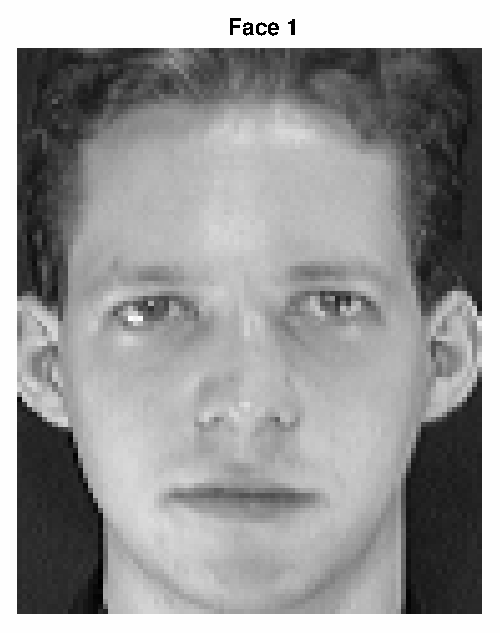
\includegraphics[scale=0.5]{./img/part_1_face}
    \caption{Part 1: att\_faces/s1/1.pgm}
    \label{fig:part_1_face}
  \end{figure}

  Next, the 2-D DCT of the image was calculated using the \texttt{dct2}
  function and plotted (Figure \ref{fig:part_1_dct}).

  \begin{figure}[H]
    \centering
    \includegraphics[scale=0.5]{./img/part_1_dct}
    \caption{Part 1: DCT}
    \label{fig:part_1_dct}
  \end{figure}

  In this plot, the image is nearly all black except for the very top-left
  corner. In order to visualize the 2-D DCT plot, the same matrix was plotted
  using a logarithmic scaled axis (Figure \ref{fig:part_1_log_dct}).

  \begin{figure}[H]
    \centering
    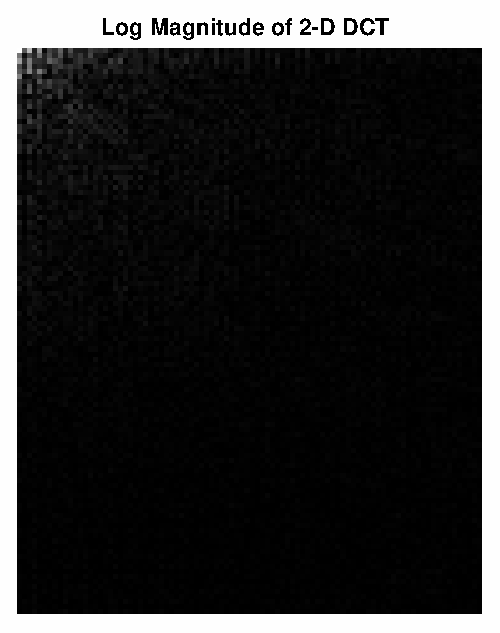
\includegraphics[scale=0.5]{./img/part_1_log_dct}
    \caption{Part 1: DCT Logarithmic Scale}
    \label{fig:part_1_log_dct}
  \end{figure}

  The logarithmic plot shows a concentration if white pixels in the top-left
  corner implying, that the DCT coefficients with the greatest magnitudes in the
  image are in the lowest-frequencies \cite{neural}.
  \\
  In order to demonstrate how the image can be recovered by calculating the inverse-DCT
  of the 2-D DCT matrix, the \texttt{idct2} function was used on the
  transform and the result was plotted (Figure \ref{fig:part_1_recovery}).

  \begin{figure}[H]
    \centering
    \includegraphics[scale=0.5]{./img/part_1_recovery}
    \caption{Part 1: Recovered Image}
    \label{fig:part_1_recovery}
  \end{figure}

  The resultant matrix matches the original image, demonstrating that the 2-D
  DCT matrix holds the same signal information as the original image matrix and
  can be used in feature extraction.

\subsection{Part 2: Feature Extraction}

  Two MATLAB\texttrademark{} scripts (Listings \ref{lst:part_2} and
  \ref{lst:findfeatures}) were used to explore feature extraction and how 2-D
  DCT of facial images can be used to discriminate between subjects. The
  \texttt{findfeatures.m} script generates a discrete signal from an image by
  first converting the 2-D matrix into a 1-D vector using zigzag 1-dimension
  reduction (Figure \ref{fig:zigzag}).
  \begin{figure}[H]
    \centering
    \includegraphics[scale=0.2]{./img/zigzag.png}
    \caption{ZigZag 1-Dimension Reduction \cite{digital video}}
    \label{fig:zigzag}
  \end{figure}

  Next, this 1-D vector is applied a discrete cosine transform and returned. The
  dimensions of the result vector is configured with the \texttt{dctlength}
  parameter, the greater this value, the more DCT coefficients are returned.
  \\
  In order to visualize the signals generated from \texttt{findfeatures},
  subject \#3's images were loaded into the \texttt{findfeatures} function and
  the output signal of each image was plotted and overlayed to show the common
  shape of the signal that subject \#3's images generate. This process was
  repeated three times while varying \texttt{dctlength} in order to show how
  increasing the amount of DCT affects the result outputted (Figures
  \ref{fig:part_2_s_3_dct_9}, \ref{fig:part_2_s_3_dct_35}, and
  \ref{fig:part_2_s_3_dct_100}).

  \begin{figure}[H]
    \centering
    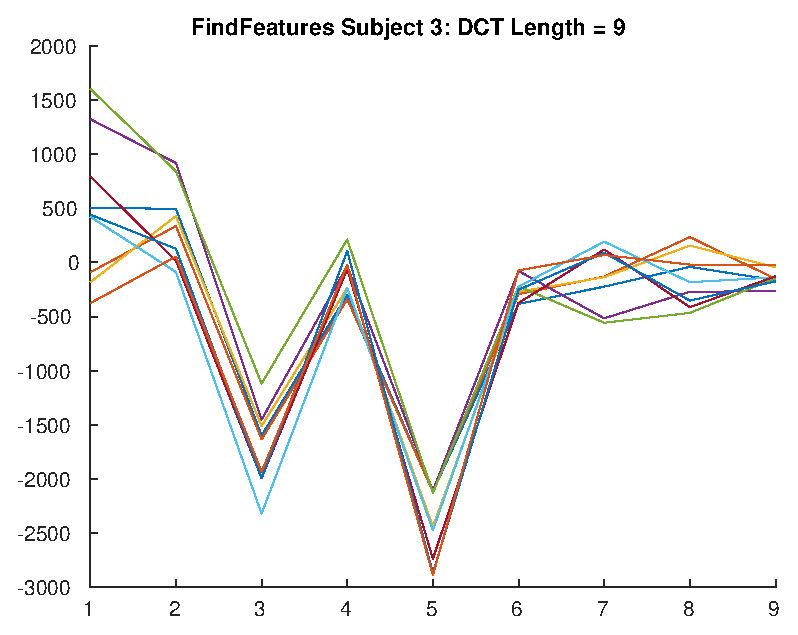
\includegraphics[scale=0.5]{./img/part_2_s_3_dct_9.eps}
    \caption{Part 2: Subject 3, DCT Length = 9}
    \label{fig:part_2_s_3_dct_9}
  \end{figure}

  \begin{figure}[H]
    \centering
    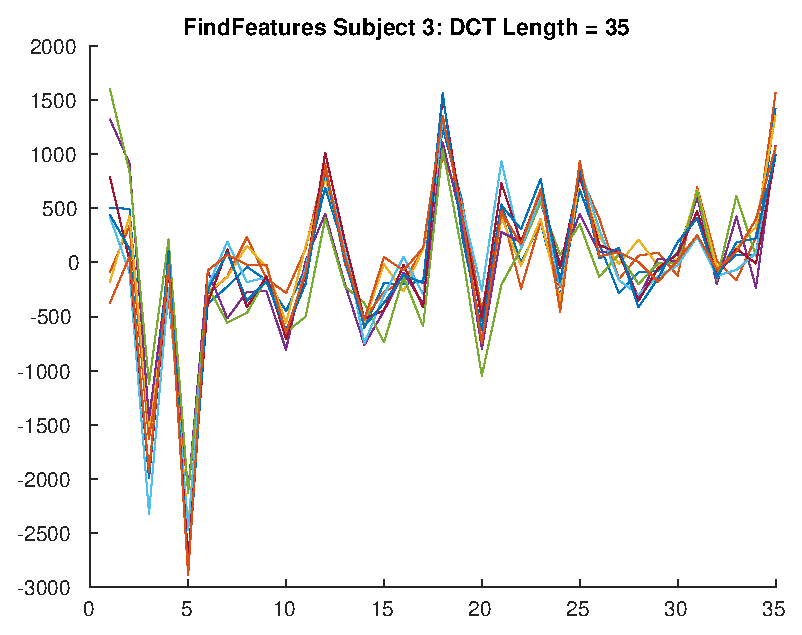
\includegraphics[scale=0.5]{./img/part_2_s_3_dct_35.eps}
    \caption{Part 2: Subject 3, DCT Length = 35}
    \label{fig:part_2_s_3_dct_35}
  \end{figure}

  \begin{figure}[H]
    \centering
    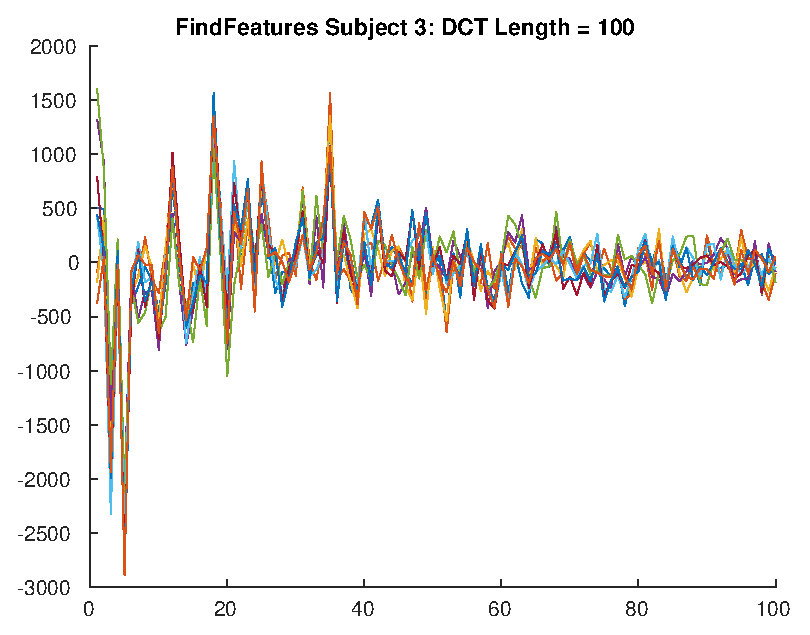
\includegraphics[scale=0.5]{./img/part_2_s_3_dct_100.eps}
    \caption{Part 2: Subject 3, DCT Length = 100}
    \label{fig:part_2_s_3_dct_100}
  \end{figure}


  Next, this same procedure was applied to another subject in order to determine
  how this method can be used to differentiate between different subjects (Figures
  \ref{fig:part_2_s_4_dct_9}, \ref{fig:part_2_s_4_dct_35}, and
  \ref{fig:part_2_s_4_dct_100}).

  \begin{figure}[H]
    \centering
    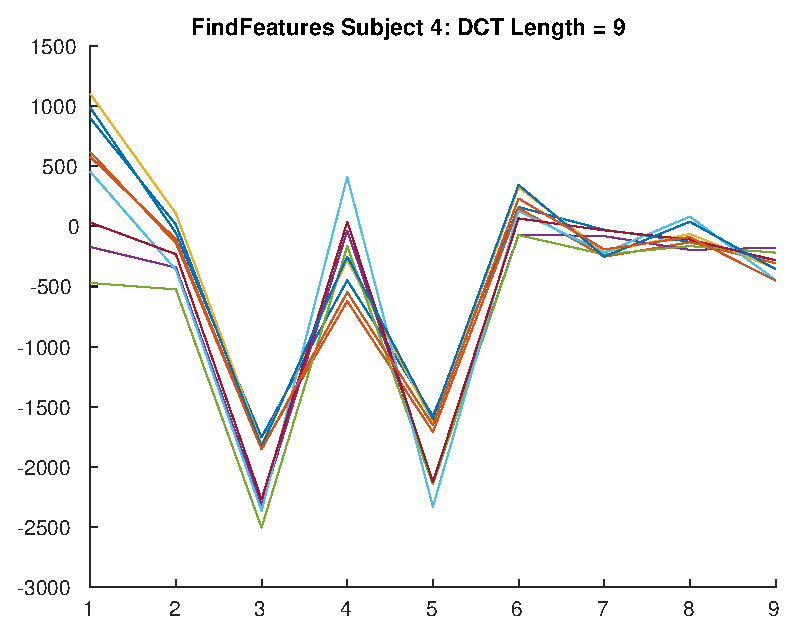
\includegraphics[scale=0.5]{./img/part_2_s_4_dct_9.eps}
    \caption{Part 2: Subject 4, DCT Length = 9}
    \label{fig:part_2_s_4_dct_9}
  \end{figure}

  \begin{figure}[H]
    \centering
    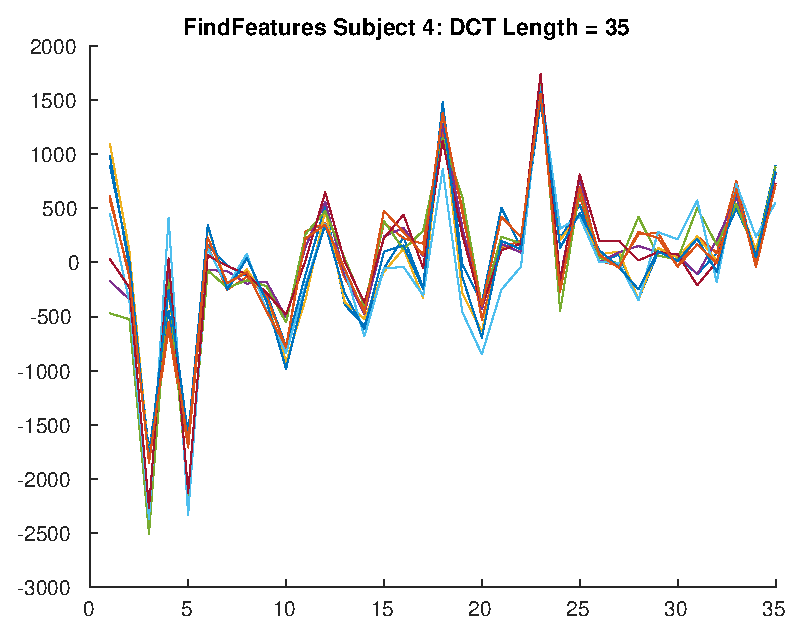
\includegraphics[scale=0.5]{./img/part_2_s_4_dct_35.eps}
    \caption{Part 2: Subject 4, DCT Length = 35}
    \label{fig:part_2_s_4_dct_35}
  \end{figure}

  \begin{figure}[H]
    \centering
    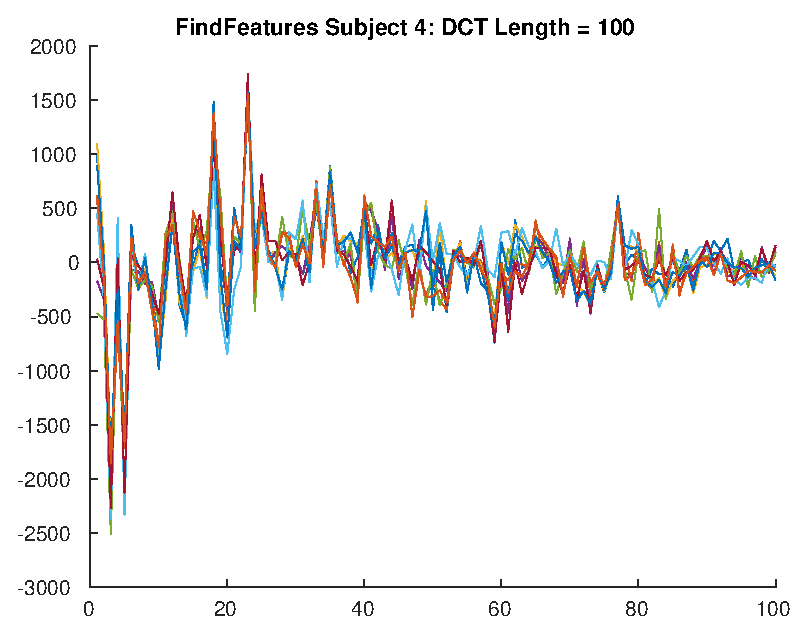
\includegraphics[scale=0.5]{./img/part_2_s_4_dct_100.eps}
    \caption{Part 2: Subject 4, DCT Length = 100}
    \label{fig:part_2_s_4_dct_100}
  \end{figure}

  The results of this test showed that facial images taken of the same subject
  will produce similar 1-D DCT signals that differ from the signals generated
  from another subject's 1-D DCT. Thus, property can be used to in image
  classification to discriminate between images of different subjects. These
  plots also reveal that descrimination becomes more apparent as the number of
  DCT coefficients increases because the signals become more unique as
  \texttt{dctlength} increases.

\subsection{Part 3: Training the Face Identification System}

In this portion of the project, a MATLAB\texttrademark{} script (Listing:
\ref{lst:part_3}) was developed to run \texttt{face\_recog\_knn\_train.m}, a
script that combines one-half of the 1-D DCT of the test images together, along
with their corresponding subject label (\texttt{trclass}) in order to create a
\texttt{trdata\_raw.mat} file that can be used in the classification of the
other half of the test images. The \texttt{face\_recog\_knn\_train.m} function
generates the trained data based on the range of subjects inputted as well as
the \texttt{dctlength} desired. Ultimatley, this \texttt{trdata\_raw.mat} data
will be used to find the closest subject DCT signal to a test image in the face
identification system in Part 4.

\subsection{Part 4: Performance Evaluation of the Face Identification System}

The final stage of this project was incorporating all of the knowledge gained in
the previous steps to develop a custom face identification system. The method
developed used the resultant \texttt{trdata\_raw.mat} from
\texttt{face\_recog\_knn\_train.m} in order to generate a 200xN matrix, where N
is the desired \texttt{dctlength}. The identification system
MATLAB\texttrademark{} scripts developed (Listings \ref{lst:part_4} and
\ref{lst:classifyFaces} used k nearest-neighbor as the basis of classifying
test images as belonging to a certain subject. The \texttt{classifyFaces}
algorithm worked as follows:
\begin{enumerate}
    \item
        A desired \texttt{dct\_coef} and \texttt{k} are set.
    \item
        \texttt{face\_recog\_knn\_train} is called to generate the trained
        dataset.
    \item
        Each test image file is iterated and transformed into a 1-D DCT using
        \texttt{findfeatures}
    \item
        Each row in \texttt{trdata\_raw} which corresponds to 1-D DCT of
        training data is iterated through and compared to each test image.
    \item
        The \texttt{knnsearch} function is used to find the index of the nearest
        neighbor to the test 1-D DCT vector from \texttt{trdata\_raw}. This
        index is used to find the corresponding subject number. This step
        is repeated $k$-times and the classes of the $k$ nearest neighbors are added to a
        vector.
    \item
        The mode of the $k$ nearest neighbor vector is taken to find which class
        occurs the most in the $k$ set and this class is used to classify the
        test image.
    \item
        A counter keeps track each iteration and a correct variable is
        incremented every time the classification matches the subject number.
        The final \texttt{success\_rate} is returned as the fraction of times
        that the classification system successfully classifies a test image.
\end{enumerate}

A second script (Listing \ref{lst:part_4}) is used to generate a 3-D data plot
that compares the values for \texttt{k} and \texttt{dctlength} and the resultant
\texttt{success\_rate} to find what the optimal values of these parameters yield
the greatest success (Figure \ref{fig:part_4_3d_plot}).

  \begin{figure}[H]
      \centering
      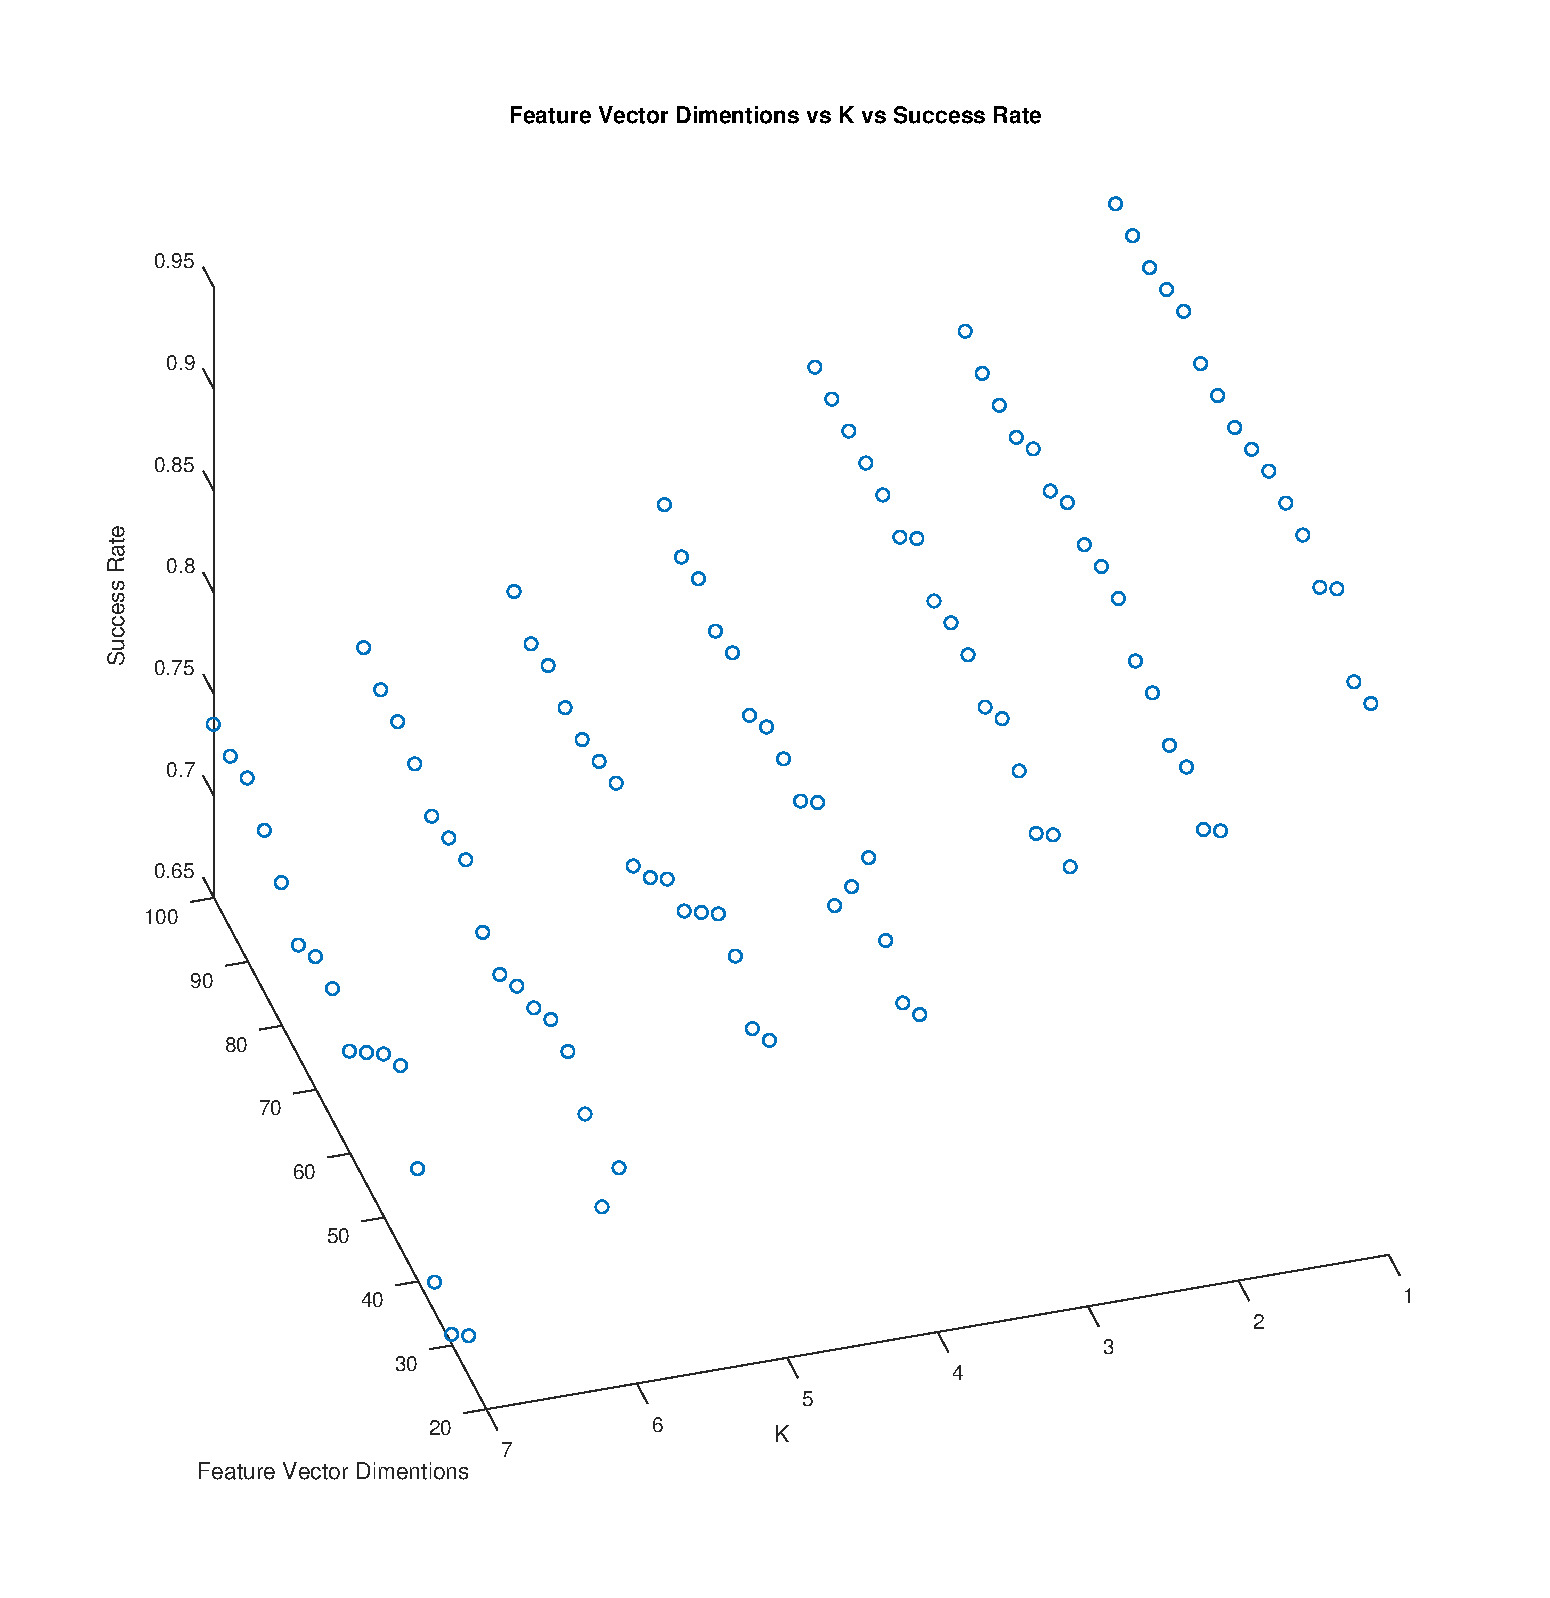
\includegraphics[scale=0.3]{./img/part_4_3d_plot.eps}
      \caption{Feature Dimensions vs K vs Success Rate}
      \label{fig:part_4_3d_plot}
  \end{figure}

  The 3-D plot determined the relationship between \texttt{k},
  \texttt{dctlength}, and \texttt{success\_rate} to be success was greatest when
  $k$ is 1 and the number of DCT dimensions was as high as possible.

\section{Summary and Conclusions}
This facial image classification project was successful in completing each of
the objectives. The final image classification system was able to achieve 96\%
classification of the 200 test images of the 40 subjects. The classification
method was able to incorporate the theory and methods used in the other three
parts to create the final system.
\\
The final classification test was able to conclude that the best discrimination
parameters is to have $k=1$ and the greatest number of 1-D DCT dimensions.
Additionally, this project showed that the kNN classifier algorithm is both
effective and fast as it was able to run through the 200 images, each with 100
1-D DCT dimentions in under 2 seconds and able to classify correctly within only
a 4\% margin of error.
\\
This classification system can be improved upon by exploring more classification
methods such as applying weights to certain DCT coefficients in order to use the
mode of the $k$ nearest neighbors in a more effective way, for instance, taking
into account that the first and second nearest neighbors can differ only
slightly and in which case, they would have a similar weight in the
classification process. Also, more advanced deep learning training
algorithms could also be investigated and compared to the current method to see
which method is fastest and/or most successful.

\begin{thebibliography}{99}

    \bibitem{neural}
    Y. Xiao, N. Chandrasiri, Y. Tadokoro and M. Oda, "Recognition of facial
    expressions using 2D DCT and neural network", \textit{Electronics and
      Communications in Japan (Part III: Fundamental Electronic Science)}, vol. 82, no. 7, pp. 1-11, 1999.

    \bibitem{new facial}
    Y. Xiao, L. Ma and K. Khorasani, "A New Facial Expression Recognition
    Technique using 2-D DCT and Neural Networks Based Decision Tree",\textit{The
      2006 IEEE International Joint Conference on Neural Network Proceedings}, 2006.

    \bibitem{discriminating}
    M. Peterson and M. Eckstein, "Perceptual learning of discriminating
    features for facial recognition", \textit{Journal of Vision}, vol. 6, no. 6, pp.
    154-154, 2010.

    \bibitem{k classifier}
    Y. Xu, Q. Zhu, Z. Fan, M. Qiu, Y. Chen and H. Liu, "Coarse to fine K nearest
    neighbor classifier", \textit{Pattern Recognition Letters}, vol. 34, no. 9, pp.
    980-986, 2013.

    \bibitem{digital video}
    G. Seo, J. Lee and C. Lee, "Frequency sensitivity for video compression",
    \textit{Optical Engineering}, vol. 53, no. 3, p. 033107, 2014.

    \bibitem{textbook}
    N. Bouaynaya, "Continuous-Time Signals", Rowan University, 2016.


\end{thebibliography}

\begin{appendix}



\lstinputlisting[basicstyle=\ttfamily\scriptsize,caption={part\_1.m},captionpos=b,label=lst:part_1]{../scripts/part_1.m}
\lstinputlisting[basicstyle=\ttfamily\scriptsize,caption={part\_2.m},captionpos=b,label=lst:part_2]{../scripts/part_2.m}
\lstinputlisting[basicstyle=\ttfamily\scriptsize,caption={part\_3.m},captionpos=b,label=lst:part_3]{../scripts/part_3.m}
\lstinputlisting[basicstyle=\ttfamily\scriptsize,caption={part\_4.m},captionpos=b,label=lst:part_4]{../scripts/part_4.m}
\lstinputlisting[basicstyle=\ttfamily\scriptsize,caption={classifyFaces.m},captionpos=b,label=lst:classifyFaces]{../scripts/classifyFaces.m}
\lstinputlisting[basicstyle=\ttfamily\scriptsize,caption={findfeatures.m},captionpos=b,label=lst:findfeatures]{../scripts/findfeatures.m}
\lstinputlisting[basicstyle=\ttfamily\scriptsize,caption={face\_recog\_knn\_train.m},captionpos=b,label=lst:face_recog_knn_train]{../scripts/face_recog_knn_train.m}

\end{appendix}

\end{document}
